\documentclass[lettersize,journal]{IEEEtran}
\usepackage{amsmath,amsfonts,amssymb}
% \usepackage{cuted}
\usepackage{algorithmic}
\usepackage{array}
\usepackage[caption=false,font=normalsize,labelfont=sf,textfont=sf]{subfig}
\usepackage{textcomp}
\usepackage{stfloats}
\usepackage{url}
\usepackage{verbatim}
\usepackage{hyperref}
\usepackage{graphicx}
\hyphenation{op-tical net-works semi-conduc-tor IEEE-Xplore}
\def\BibTeX{{\rm B\kern-.05em{\sc i\kern-.025em b}\kern-.08em
    T\kern-.1667em\lower.7ex\hbox{E}\kern-.125emX}}
\usepackage{balance}
\bibliographystyle{IEEEtran}
\graphicspath{ {./images/} }


\begin{document}
\title{Nonreciprocity in the system of two superconducting qubits coupled to a 1D waveguide: influence of higher energy levels and quantum correlations}
\author{Nikita Nefedkin, Andrea Al{\`u} \IEEEmembership{Fellow, IEEE}
\thanks{Nikita Nefedkin (nnefedkin@gc.cuny.edu) is with the Advanced Science Research Center, City University of New York, New York, New York, 10031, USA.}
\thanks{Andrea Al\`u (aalu@gc.cuny.edu) is with the Advanced Science Research Center and Graduate Center, City University of New York, New York, New York, 10031, USA.}}

\markboth{Journal of \LaTeX\ Class Files,~Vol.~18, No.~9, September~2020}%
{How to Use the IEEEtran \LaTeX \ Templates}

\maketitle

\begin{abstract}
This paper delves into the intricacies of nonreciprocity in a system composed of two superconducting qubits operating in a transmon regime and coupled to a one-dimensional (1D) waveguide. Nonreciprocity, characterized by asymmetrical signal transmission and reflection, is a phenomenon of increasing interest in quantum technologies. Our investigation focuses on how theoretical approximations impact observed nonreciprocal effects and highlights crucial factors that must be considered. By employing the real parameters of the qubits, we uncover significant alterations in system dynamics when higher energy levels are included in the transmon regime. This leads to a reduction in nonreciprocity, with the diode efficiency falling below the two-level approximation limit of $2/3$. Additionally, the statistical properties of the system undergo significant changes, particularly in the coherent functions for transmitted and reflected signals. The emergence of additional population transfer channels and the critical role of quantum correlations between qubits underscore the necessity of precise modelling. These findings have direct implications for quantum device engineering, offering insights that can enhance the design of more efficient quantum devices and advanced quantum communication systems.
\end{abstract}

\begin{IEEEkeywords}
Superconducting qubits, nonreciprocity, subradiance, quantum correlations
\end{IEEEkeywords}


\section{Introduction}

\IEEEPARstart{S}{uperconducting} qubits have established themselves as a potential platform for constructing nonreciprocal devices in the field of quantum technologies~\cite{rosario_hamann_nonreciprocity_2018, gheeraert2020programmable, rymarz2021hardware, kutsaev2021up, redchenko2023tunable}. These qubits, characterized by their convenience and controllability, hold significant promise for applications in quantum information processing and quantum device engineering. The pursuit of efficient and precise manipulation of quantum states, signal routing and processing necessitates a profound understanding of nonreciprocal behaviour in such systems.

Nonreciprocity, characterized by the non-symmetrical response of a system to signal transmission and reflection, has garnered considerable attention in recent years~\cite{caloz2018electromagnetic,nassar2020nonreciprocity,manipatruni2009optical, mahoney2017chip,zhang2018thermal, rosario_hamann_nonreciprocity_2018, nefedkin_nonreciprocal_2023}. Previous studies have highlighted its potential in quantum signal routing, amplification, and information processing~\cite{Furnkranz2020Quantum, Kimble2008quantum}. However, the extent to which theoretical approximations influence observed nonreciprocal effects and the critical factors that demand consideration for accurate modelling remain areas of active investigation.

This work delves into the intricacies of nonreciprocal quantum systems, with a particular focus on a system comprising two superconducting qubits operating in a transmon regime, coupled to a one-dimensional (1D) waveguide~\cite{dai_rectification_2015, muller_nonreciprocal_2017, rosario_hamann_nonreciprocity_2018, Nefedkin2022}. The primary objective is to scrutinize the impact of theoretical approximations on nonreciprocal phenomena and to delineate the essential factors governing these effects.

In this study, we employ the real parameters of the qubits obtained from ref.~\cite{rosario_hamann_nonreciprocity_2018}. Utilizing them, we explore the dynamics of a system with the potential for nonreciprocity. Usually, explanations of the mechanism of the nonreciprocity emergence are grounded in the simplified two-level qubit model~\cite{lalumiere_input-output_2013, muller_nonreciprocal_2017}. In this model, two one-excitation states, dark and bright, are populated differently depending on the direction of excitation. In one scenario, constructive interference between the population transfer channels involving ground, bright, and dark states leads to the population of the dark state and, consequently, an increase in the intensity of the transmitted signal. In the other case, destructive interference among these channels results in all states, except the ground state, remaining unpopulated, causing the signal to be fully reflected. It is the interplay between these two behaviours that gives rise to the nonreciprocity of the system. 

Transitioning into a transmon regime characterized by weak anharmonicity~\cite{krantz_quantum_2019}, the potential impact of higher energy levels within the qubits becomes a pivotal consideration. Within this regime, our investigation reveals a notable shift in the system's behaviour, notably a reduction in nonreciprocity, exemplified by a substantial decrease in the nonreciprocity (diode) efficiency, falling below the conventional two-level system limit of $2/3$~\cite{muller_nonreciprocal_2017}. This phenomenon is intrinsically tied to the intricate quantum dynamics of the system, which is comprehensively explored in this study.

This behaviour is attributed to the emergence of two additional population transfer channels associated with symmetric and antisymmetric qubit states with two excitations. These channels come into play under moderate incident powers, where they interfere destructively with the existing channels, ultimately diminishing the nonreciprocity effect. Importantly, this phenomenon persists even when considering more than three energy levels of the qubits, although with minor quantitative variations in populations, transmissions, and reflections.

Furthermore, our investigation underscores the pivotal role of accounting for quantum correlations between the qubits to model the nonreciprocity effect accurately. Conventional semiclassical models, relying on factorized expectation values of operator products, inadequately capture the system's dynamics in some scenarios~\cite{carmichael1999statistical}. This deficiency is primarily due to the emergence of strong correlations, such as $\langle \sigma_j^+ \sigma_k \rangle$ for $j\neq k$, which become prominent in the nonreciprocal regime. Notably, these correlations diminish at lower incident powers, thereby rendering the semiclassical approximation applicable in this regime.

The insights derived from this investigation bear profound implications for the field of quantum device engineering. A comprehensive understanding of the relationship between theoretical approximations and nonreciprocal effects paves the way for developing more efficient and versatile quantum devices, particularly in the context of quantum diodes and signal processing. Moreover, the emphasis on precision in modelling is a valuable asset in advancing the design and implementation of advanced quantum communication systems. By elucidating these findings in greater detail, this paper aims to provide a thorough analysis of the system, the mathematical models utilized, and the empirical outcomes.


\section{Two superconducting qubits coupled to a 1D waveguide: theoretical description}
\noindent The system of two qubits coupled to a 1D waveguide has been vastly studied theoretically in Refs.~\cite{muller_nonreciprocal_2017, dai_rectification_2015, Nefedkin2022, trivedi_fano-qubits_2023, lalumiere_input-output_2013} and experimentally in Refs.~\cite{rosario_hamann_nonreciprocity_2018}. 
In most theoretical works, the waveguide degrees of freedom are adiabatically excluded, and the effective Hamiltonian describes qubits interacting with each other through the Green's tensor of the waveguide.
Excitations in the waveguide are considered to be in a coherent state and can be treated classically.
We use this approach in this work and derive an effective Hamiltonian and the master equation, eliminating the waveguide degrees of freedom.
However, here, we consider the description of the transmon qubits based on their circuit representation.

A typical superconducting qubit circuit consists of two main elements: the Josephson junction~\cite{Josephson1962Possible} subcircuit and the shunt capacitance, $C_S$, connected in parallel, see Fig.~\ref{fig:01}(a). 

\begin{figure}[h]
    \centering
    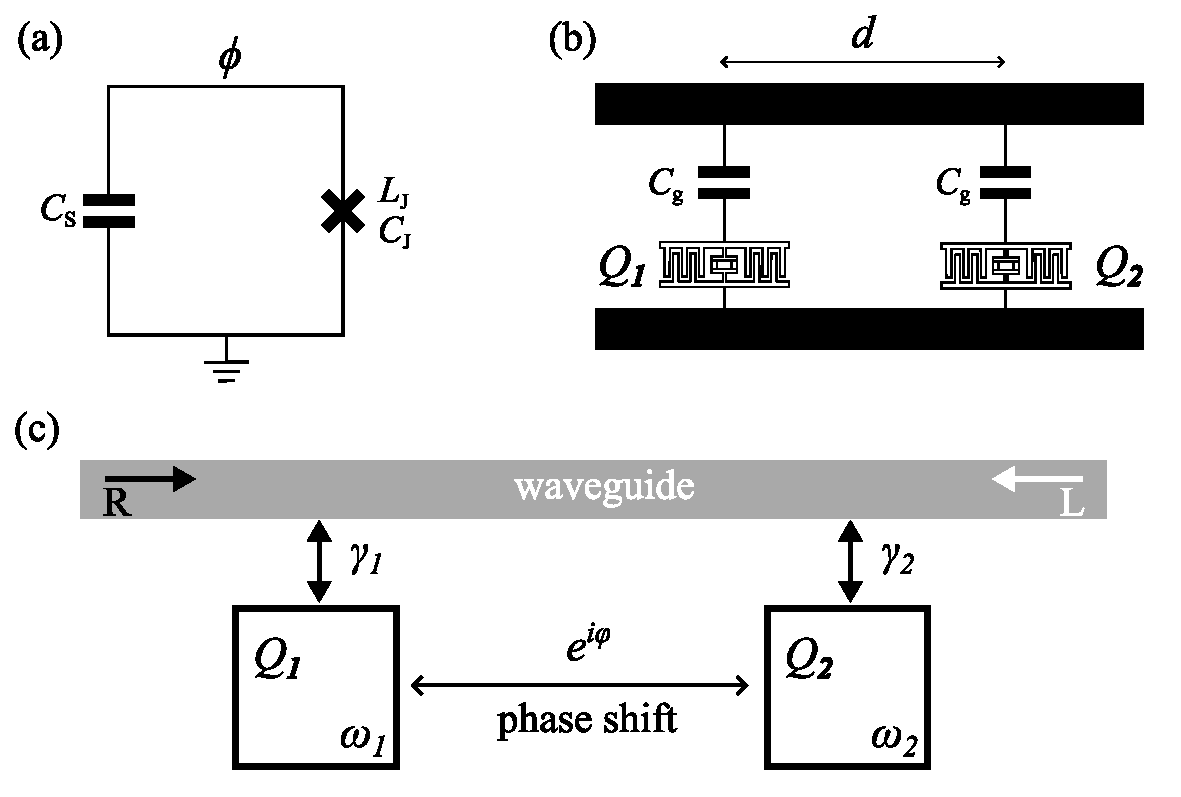
\includegraphics[width=0.45\textwidth]{fig_1}
    \caption{(a) Qubit circuit with nonlinear inductance $L_J$ and shunt capacitance $C_S$; (b) schematic representation of two transmon qubits coupled to a 1D waveguide line; (c) sketch of the system described by the effective Hamiltonian.}
    \label{fig:01}
\end{figure}

The Josephson junction subcircuit is characterized by the junction inductance $L_J$ and the junction self-capacitance, $C_J$, which is usually much larger (for the conventional circuit designs)~\cite{krantz_quantum_2019}.
The Hamiltonian of the qubit, Fig.~\ref{fig:01}, is written in generalized circuit coordinates, namely, the node flux $\Phi$ and the capacitor charge $Q$, after canonical quantization~\cite{}.
It has the form:
\begin{equation}\label{eq:01}
    H = 4 E_C N^2 - E_J \cos \phi,
\end{equation}
where $E_C = e^2 / (2 (C_J + C_S))$ is the charging energy required to add an electron from the Couper pair to the superconducting island; $N$ is the number of Cooper pairs in the island; conjugate to the junction superconducting phase difference $\phi$; $E_J = I_c \Phi_0 / 2\pi$ is the Josephson energy with $\Phi_0 = h / 2e$ being the magnetic superconducting flux and $I_c$ being the critical current of the junction.
The Josephson energy is connected to the nonlinear inductance of the junction $L_J$ through the following relation: $L_J^{_1} = (2e^2 / \hbar)^2 d^2(E_J \cos \phi) / d\phi^2 = (2e^2 / \hbar)^2 E_J \cos \phi$. 
The eigenstates of the Hamiltonian (\ref{eq:01}) are shown in Fig.~\ref{fig:02}(a).

\begin{figure}[h]
    \centering
    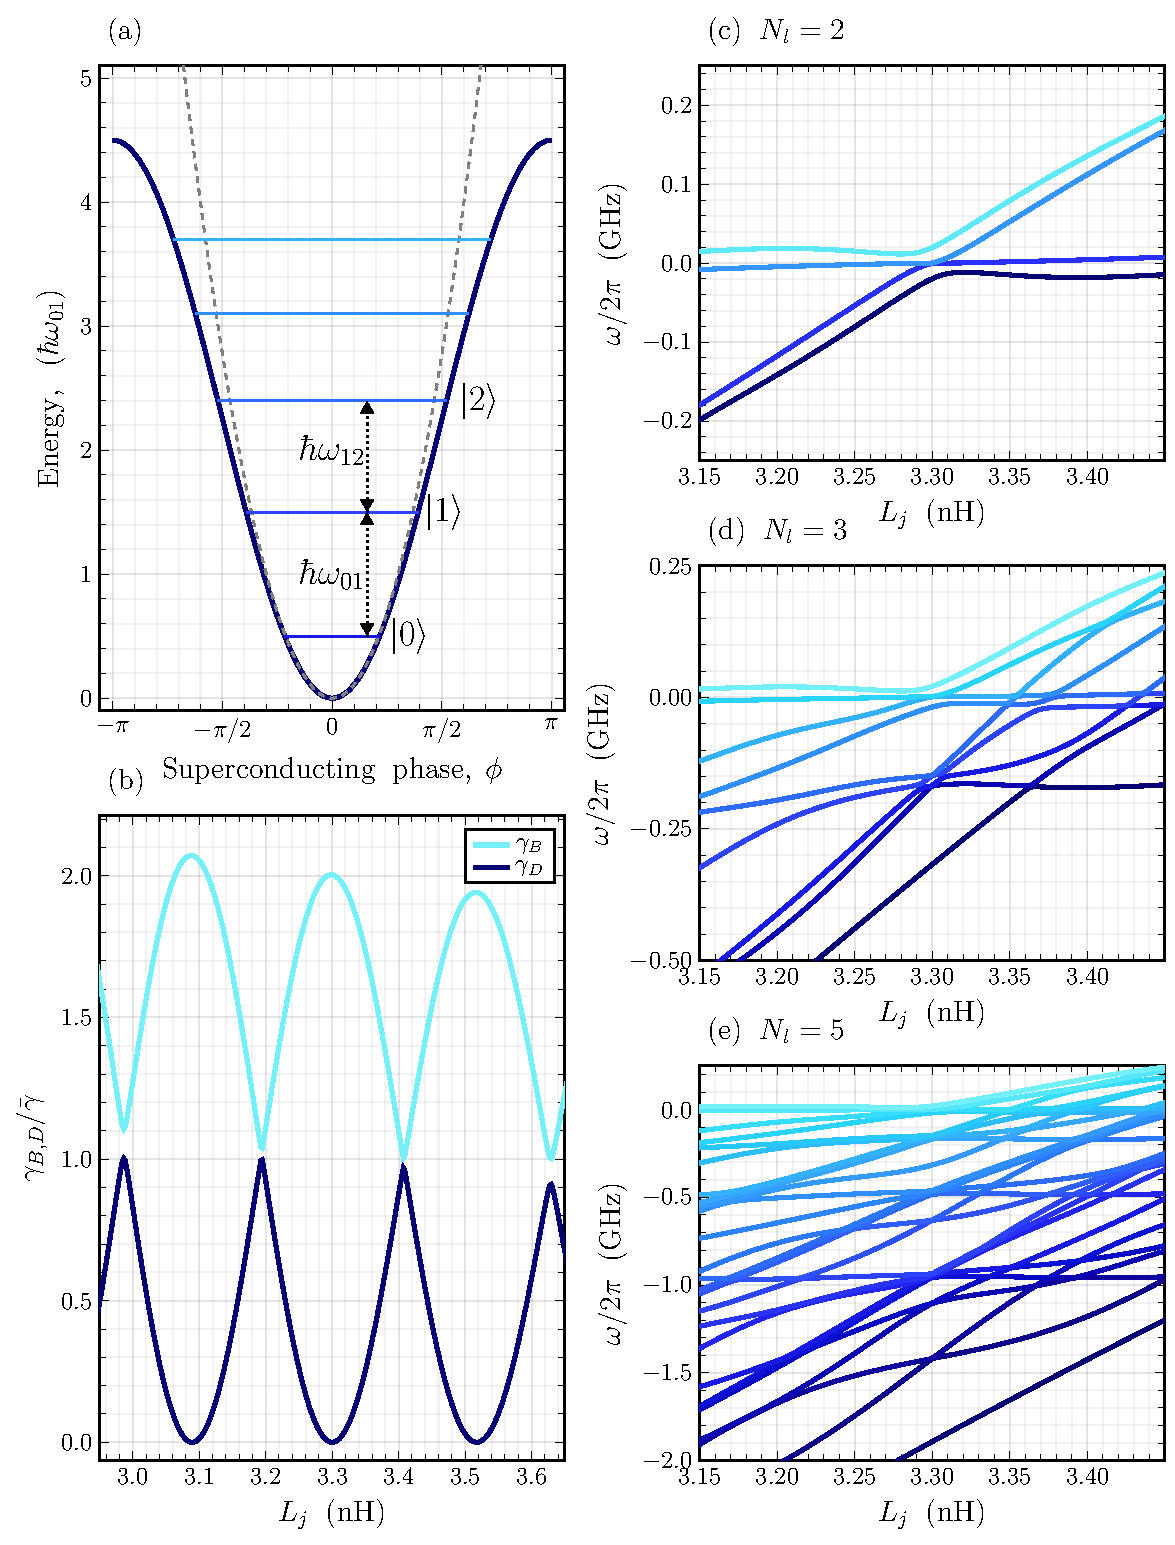
\includegraphics[width=0.45\textwidth]{fig_2}
    \caption{(a) Eigenenergies of a transmon qubit depicted in Fig.~\ref{fig:01}; (b) dark and bright state decay rates normalized by the average decay rate of the qubits to a waveguide at $L_J^{(1)} = L_J^{(2)}$; eigenenergies of the system of two qubits coupled to a waveguide depending on the nonlinear inductance of the Josephson junction for different number of qubit levels considered: two levels (c), three levels (d) and five levels (e).}
    \label{fig:02}
\end{figure}

\subsection{Two limits and the transmon regime}

The Hamiltonian (\ref{eq:01}) may be analyzed under two distinct limits: $E_J \ll E_C$ and $E_J \gg E_C$.
In the first limit, $E_J \ll E_C$, we encounter a regime characterized by strong charge quantization, resulting in Coulomb blockade oscillations. 
This regime, called the Cooper pair box regime, exhibits a significant charge dispersion effect in the qubit frequency. This dispersion is a consequence of the pronounced dependence of charge eigenenergies on gate potential, resulting in a heightened susceptibility of the qubit to charge-induced noise.

In the contrasting regime where $E_J \gg E_C$, commonly called the transmon regime, quantum fluctuations suppress charge quantization. 
This suppression results in an exponential reduction in charge dispersion. Consequently, the susceptibility of the qubit to noise experiences a pronounced diminishment, leading to a noteworthy increase in quantum coherence.
However, this increased quantum coherence is accompanied by the trade-off of reduced anharmonicity. 
In the transmon regime, the qubit spectrum closely approximates a harmonic behaviour, with the frequency determined by the Josephson plasma frequency, $\omega_{pl} = \sqrt{8 E_J E_C} / \hbar$.
This diminished anharmonicity, in turn, translates into shorter operation times due to the leakage out of the qubit subspace.

\subsection{Taylor series of the potential and anharmonicity}

The cosine potential of the Josephson junction with Josephson energy $E_J$ can be Taylor expanded to order $m$ for small values of its phase fluctuations $\phi$ across it:
\begin{equation} \label{eq:02}
   V(\phi) = - E_J \cos \phi = \sum_{m > 0} \frac{(-1)^{m} \phi^{2m}}{(2m)!}.
\end{equation}
The first term within the series is quadratic, giving rise to the eigenvalues and eigenfunctions of a quantum harmonic oscillator.
The subsequent term, being quadric, introduces modifications to the eigensolutions and perturbs the harmonic energy structure.
It is worth noting that the presence of a negative coefficient in the quartic term implies that the anharmonicity $\alpha = \omega_{12} - \omega_{01}$, which represents the difference in frequency between the lowest two energy levels and the subsequent two, is inherently negative. 
Consequently, its maximum magnitude cannot be arbitrarily increased. 
In the context of the transmon qubit, $\alpha$ is typically engineered to be within the range of 100–300 MHz, where $\alpha = -E_C$.

\subsection{Second quantization}

Usually, it is more convenient to work in occupation number representation.
Keeping the terms up to the fourth order in the Josephson potential (\ref{eq:02}) and conducting the second quantization procedure of the Hamiltonian (\ref{eq:01}) using the following ansatz: $N \propto i(a - a^\dag)$ and $\phi \propto (a + a^\dag)$, we arrive to the second-quantized Hamiltonian of the form:
\begin{equation} \label{eq:03}
    H = \hbar \omega_q a^\dag a + \frac{\alpha}{2} a^\dag a^\dag a a
\end{equation}
As mentioned above, $|\alpha| \ll \omega_q$ leads to a quasiharmonic eigenenergy structure and can cause leakage out of the qubit subspace, increasing the operation errors.
However, several strategies in the transmon regime are employed to mitigate leakage out of the qubit subspace, including design improvements, asymmetric transmons, dynamical error suppression exploiting the 1/x distribution of flux noise, and cryogenic engineering. 
These methods collectively aim to enhance qubit performance by reducing sensitivity to noise sources and bolstering coherence and fidelity during qubit operations.
If we managed to separate two-level subspace from higher levels, we could treat the qubit as a two-level system (TLS), and the Hamiltonian becomes:
\begin{equation} \label{eq:03_1}
    H = \hbar \omega_q \frac{\sigma_z}{2},
\end{equation}
where $\sigma_z = |1\rangle\langle 1 | - | 0 \rangle \langle 0|$ is a Pauli-z operator.

\subsection{Hamitonian of the system}

Hamiltonian (\ref{eq:03}) describes a qubit in occupation number representation.
This work considers a system of two transmon qubits at a distance $d$ (with coordinates $x_1 = 0$ and $x_2 = d$, correspondingly)  coupled to a transmission line (1D waveguide); see Fig.~\ref{fig:01}(b).
The time required for the field to propagate to the qubit $j$ is $t_j = x_j / v$, where $v$ is the field propagation speed.
The total Hamiltonian of the system includes the qubit Hamiltonians, the waveguide Hamiltonian for right- and left-propagating modes and their interaction Hamiltonian.
It takes the form:
\begin{align} \label{eq:04}
    H_Q &= \hbar \sum_j \left( \omega_j a_j^\dag a_j + \frac{\alpha}{2} a_j^\dag a_j^\dag a_j a_j \right), \\
    H_W &= \hbar \int_0^\infty d \omega \omega \left( a_R^\dag(\omega) a_R(\omega) + a_L^\dag(\omega) a_L(\omega) \right), \\
    H_I &= \hbar \sum_j g_j (\Omega_j + \Omega_j^+) (a_j + a_j^\dag), \\
    H &= H_Q + H_W + H_I,
\end{align}
where $\omega_j$ is the transition frequency of the $j$th qubit; $a_{R/L}(\omega)$ is the bosonic annihilation operator of the right/left propagating photon in the waveguide; $g_j$ is the dimensionless coupling constant between the field in the waveguide and the $j$th qubit; $\Omega_j = - i \int_0^\infty d \omega \sqrt{\omega} \left( a_L(\omega) e^{-i \omega x_j / v} + a_R(\omega) e^{i \omega x_j / v} \right)$ is an incident field amplitude at the position of the $j$th atom.
Note that, to derive this simplified form for $H_W$ and $H_I$, we have assumed that the waveguide dispersion is linear around a particular frequency of interest $\omega_0$, that is, $\omega(k) \approx \omega_0 + v (k - k_0)$, so that the wavevector of the guided mode is $k(\omega) \approx k_0 + (\omega - \omega_0) / v$~\cite{shen_theory_2009} and the common terms $k_0$ and $\omega_0/v$ can be re-absorbed in the definition of $a_L$ and $a_R$.

\subsection{Effective Hamiltonian}

The Hamiltonian (\ref{eq:04}) describes the entire waveguide-atom system. Still, using it for analytical and numerical calculations is cumbersome because it explicitly contains the infinite degrees of freedom associated with the waveguide modes.
Suppose we are not interested in the dynamics of these modes. 
In that case, it is possible to "trace out" the waveguide degrees of freedom and obtain an effective finite-dimensional master equation describing only the evolution of the qubits. 
This procedure is described in Refs.~\cite{gardiner2004quantum,lehmberg_radiation_1970,lalumiere_input-output_2013}. 
We also assume that the waveguide field incident from two directions is monochromatic and is in a coherent state, with amplitudes $a_{in}^{R/L}$ and driving frequency $\omega_d$. 
Under a Markov and rotating wave approximation, we obtain the master equation for the reduced density matrix:
\begin{equation} \label{eq:05}
    \dot{\rho} = \frac{i}{\hbar} \left[ H_\mathrm{eff}, \rho \right] + \sum_{j,k} \frac{\Gamma_{jk}}{2} \left( 2 a_j \rho a_k^\dag - \rho a_k^\dag a_j - a_k^\dag a_j \rho \right)
\end{equation}
with the effective Hamiltonian of the form:
\begin{align} \label{eq:06}
    H_\mathrm{eff} =& \hbar \sum_j \left( (\omega_j - \omega_d) a_j^\dag a_j + \frac{\alpha}{2} a_j^\dag a_j^\dag a_j a_j \right) + \nonumber \\
    &\hbar \sum_j \left\{ -2 \sqrt{\frac{\gamma_j}{2}} \sqrt{\frac{\omega_d}{\omega_j}} \left[ a_\mathrm{in}^L \sin(\omega_d (t + t_j)) + \right.\right.\\
    &\left.\left.a_\mathrm{in}^R \sin(\omega_d (t - t_j)) \right] e^{-i \omega_d t} a_j + \mathrm{h.c.} \right\} + \nonumber \\
    &\hbar \sum_{jk} \Omega_{jk} a_j^\dag a_k \nonumber
\end{align}
The first sum describes the individual qubits, as we showed in Eq. (\ref{eq:04}).
The second sum is a driving term describing coupling the qubits to the waves in the waveguide.
The last sum is responsible for qubit-qubit effective interaction through the waveguide.
Here, $\Gamma_{jj} = \gamma_j$ is the decay rate of the individual qubit to the waveguide, and $\Gamma_{jk} = \sqrt{\gamma_j \gamma_k}/2 \left( \sqrt{\omega_j / \omega_k} e^{i \omega_j t_{kj}} +  \sqrt{\omega_k / \omega_j} e^{-i \omega_k t_{jk}}\right)$, $j\neq k$ is the correlated decay rate of the qubits.
$\Omega_{jk} = -i\sqrt{\gamma_j \gamma_k}/4 \left( \sqrt{\omega_j / \omega_k} e^{i \omega_j t_{kj}} -  \sqrt{\omega_k / \omega_j} e^{-i \omega_k t_{jk}} \right)$, $j\neq k$ is the amplitude of exchange interaction between the qubits being mediated by virtual excitations in the waveguide.
The phase of the right propagating (R) or left propagating (L) wave at the position of the $j$th qubit is $\varphi_j^{R/L} \equiv \mp \omega_d x_j / v$.
Note that in the master equation (\ref{eq:05}), we do not consider dephasing processes and nonradiative losses. 
These losses and their impact on the system's behaviour were considered in, e.g., refs.~\cite{rosario_hamann_rectangular_2019, Nefedkin2022}.

\subsection{Realistic qubit system and $L_J$ dependence}

In this work, we start from the electric circuit description of the qubits with realistic parameters close to the ones from ref.~\cite{rosario_hamann_nonreciprocity_2018}.
We use the open-source library QuCAT~\cite{gely_qucat_2020} to model the qubits and obtain their parameters.
We consider two qubits depicted in Fig.~\ref{fig:01}(a,b) with the following parameters: $C_S = 63$ fF, $C_g = 60$ fF, the impedance of the waveguide $Z = 5 \; \mathrm{\Omega}$, the nonlinear inductance of qubit 2 is fixed and equals $L_J^{(2)} = 3.3$ nH, the nonlinear inductance of qubit 1 can vary and thereby change the eigenfrequency of the qubit $\Delta \omega_q = - \left( \frac{\Phi_0}{2 \pi} \right) \frac{\sqrt{2 E_C}}{\hbar L_J^{3/2}} \Delta L_J$, however, to create the detuning corresponding to the one from ref.~\cite{rosario_hamann_nonreciprocity_2018}, $L_J^{(1)} = 3.31$ nH.
These parameters give the following frequencies, decay rates and anharmonicities:
\begin{table}[h!]
\centering
\caption{Parameters of the transmon qubits.}
\begin{tabular}{||m{1cm} m{1.6cm} m{1.6cm} m{1.6cm}||} 
 \hline
 & Frequency (GHz) & Decay rate (MHz) & Anharmonicity (MHz) \\
 \hline\hline
 Qubit 1 & 7.89 & 81.3 & 158 \\
 \hline
 Qubit 2 & 7.9 & 81.5 & 158 \\
 \hline
\end{tabular}
\label{tab:01}
\end{table}
Thus, $|\alpha| \ll \omega_j$, and we can see that the qubit works in the transmon regime.

In the present work, we consider the system of two qubits coupled to a waveguide in the context of breaking Lorentz reciprocity (or the nonreciprocity effect)~\cite{}.
It was shown in refs.~\cite{dai_rectification_2015,muller_nonreciprocal_2017,rosario_hamann_nonreciprocity_2018, Nefedkin2022} that in such a system under certain conditions, the transmission of the waves propagating in one direction is much larger than the transmission in the other direction.
Breaking Lorentz reciprocity in passive systems (without external magnetic bias or modulation) requires from the system two key characteristics: (i) the system must be nonlinear; (ii) the system's inversion symmetry must be broken~\cite{}.
In the system under our consideration, nonlinearity naturally emerges due to anharmonicity, whereas broken inversion symmetry can be created by detuning one of the qubits.
We consider the incident wave frequency to be in resonance with the transition frequency of the second qubit, i.e., $\omega_d / 2\pi = 7.9$ GHz.
As mentioned above and shown in Tab.~\ref{tab:01}, to break the inversion symmetry in the system, we consider a small detuning of qubit 1.
This asymmetry is determined by the dimensionless parameter $\delta = \frac{\omega_1 - \omega_d}{\bar{gamma}}$, $\bar{\gamma} = (\gamma_1 + \gamma_2) / 2$.
The inter-qubit distance $d$ is chosen so that the system operates near the first Fabry–Perot resonance; that is, the single-trip accumulated phase is $\varphi = \omega_d d / v = \pi - \xi$, where $\xi$ is a small tunable phase delay. 
Following~\cite{dai_rectification_2015,muller_nonreciprocal_2017}, we set $\xi = \delta$ to compensate for the additional phase shift $-\delta$ that emerges due to small detuning of qubit 1. 
As was shown in ref.~\cite{muller_nonreciprocal_2017}, these parameters provide the optimal asymmetry in the response of the two-qubit system to form a nonreciprocal response.

In this configuration, the nonreciprocity effect is raised due to the existence of two particular states: the fast decaying bright state, $|B\rangle$, and the slow decaying dark state, $|D\rangle$.
In the basis of dark and bright states, for one direction of propagating waves in the waveguide, the bright state is populated, and due to the fast decay rate, $\gamma_B > \gamma_j$, immediately emits the photon in the reverse direction. 
Thus, the system behaves as a perfect mirror at low powers, $|a_\mathrm{in}|^2 / \gamma_B$.
For another direction of propagating waves, the dark state becomes populated, and due to the slow decay, the population is trapped in the dark state. 
The whole system becomes transparent, i.e., transmission grows.
Thus, the system demonstrates nonreciprocal behaviour when the incident wave power is constrained in the following limits: $ \gamma_D < |a_\mathrm{in}|^2 < \gamma_B$.

\subsection{Dark and bright states}

To understand better how we can obtain the decay rates of the dark and bright states and define the states, we take a closer look at the dissipation part of the master equation (\ref{eq:05}).
Following~\cite{gross1982superradiance, carmichael_quantum_2000, clemens_collective_2003}, we can diagonalize the coefficient matrix $(\Gamma_{jk})$ and go to collective operators or the source-mode jump operators form.
The general form of the source-mode jump operators is the following:
\begin{align}\label{eq:07}
    \vec{J} =& \sqrt{\mathbf{\Lambda}} \mathbf{B} \vec{\Sigma},\\
    \vec{J}^\dag =& \vec{\Sigma}^\dag \mathbf{B}^T \sqrt{\mathbf{\Lambda}},
\end{align}
where 
\begin{equation} \label{eq:08}
    \left( \Gamma_{jk} \right) = \mathbf{B}^T \sqrt{\mathbf{\Lambda}} \mathbf{B}, \;\; \mathbf{\Lambda} \equiv \mathrm{diag}(\lambda_1, \ldots, \lambda_N)
\end{equation}
\begin{equation} \label{eq:09}
    \vec{\Sigma} \equiv \left( a_1, \ldots, a_N \right)^T
\end{equation}
and $N$ is the number of qubits in the system.
Then the master equation becomes:
\begin{equation} \label{eq:10}
    \begin{aligned}
        \dot{\rho} = -\frac{i}{\hbar} \left[H_\mathrm{eff}, \rho\right] + \frac{1}{2} \sum_{m=1}^N &\left( 2 J_m \rho J_m^\dag - \right.\\
        &\left.\rho J_m^\dag J_m - J_m^\dag J_m \rho \right)
    \end{aligned}
\end{equation}

For the system of two qubits (in the formulas above $N=2$), the eigenvalues of $(\Gamma_jk)$ are the decay rates of the dark and bright states:
\begin{equation} \label{eq:11}
    \gamma_{B/D} = \frac{\gamma_1 + \gamma_2}{2} \pm \sqrt{\left(\frac{\gamma_1 - \gamma_2}{2}\right)^2 + |\gamma_{12}|^2}.
\end{equation}
The collective operators take the form:
\begin{equation} \label{eq:12}
    J_{B/D} = \sqrt{\gamma_{B/D}} \frac{(\gamma_{B/D} - \gamma_2) a_1 + \gamma_{12}^* a_2}{\sqrt{(\gamma_{B/D} - \gamma_2)^2 + |\gamma_{12}|^2}}
\end{equation}
and finally, we can find the dark and bright states.
They appear as follows:
\begin{equation}  \label{eq:13}
    \begin{aligned}
        |B/D\rangle =& \frac{\gamma_{B/D} - \gamma_2}{\sqrt{(\gamma_{B/D} - \gamma_2)^2 + |\gamma_{12}|^2}} |1,0\rangle + \\
        &\frac{\gamma_{12}}{\sqrt{(\gamma_{B/D} - \gamma_2)^2 + |\gamma_{12}|^2}} |0,1\rangle,
    \end{aligned}
\end{equation}
where the state $|n,m\rangle = |n\rangle \otimes |m\rangle$ has $n$ excitations of qubit 1 and $m$ excitations of qubit 2.

The dependence of $\gamma_D$ and $\gamma_B$ on the inductance of qubit 2, $L_J^{(2)}$, is shown in Fig.~\ref{fig:02}(b).
Near the resonance (when $\omega_1 = \omega_2 = \omega_d$ or $L_J^{(1)} = L_J^{(2)}$), the behaviour of decay rates can be approximated by the following function:
\begin{equation} \label{eq:14}
\begin{aligned}
    &\gamma_{B/D} = \gamma \left(1 \pm \left|\cos\left( \omega_d \frac{\pi - \delta}{\gamma} \right) \right| \right) = \\
    &\gamma \times \\
    &\left[ 1 \pm \left| \cos \left( \frac{\omega _d}{\gamma} \frac{\left(\hbar  \omega _d +\hbar \pi \gamma - \left( \frac{\Phi_0}{2\pi} \right) \sqrt{\frac{8 E_C}{L_J}}+E_C\right)}{\hbar \gamma}\right) \right| \right]
\end{aligned}
\end{equation}
Here we assumed that $\gamma_1 =  \gamma_2 = \gamma$.
The period of decay rate oscillations can be obtained by linearization near the resonance, i.e., near $L_J^{(2)}$:
\begin{equation} \label{eq:15}
    T_{L_J} = \frac{\sqrt{2} \pi  \gamma ^2 \hbar  L_J^{(2)}}{\left( \frac{\Phi_0}{2\pi} \right) \omega_d \sqrt{\frac{E_C}{L_J^{(2)}}}}
\end{equation}

Figs.~\ref{fig:02}(c-e) show the eigenenergies of the effective Hamiltonian (\ref{eq:06}) also depending on the Josephson inductance of qubit 1, $L_J$.
These figures show the Hamiltonians with different numbers of levels taken into account: $N_l = 2$, $N_l = 3$, and $N_l = 5$.
For the two-level case, the eigenenergies demonstrate avoided crossing behaviour.
If we increase the number of levels in the qubits, the eigenenergies picture becomes more complicated and the structure of the levels close to zero changes.
The following section considers how these differences affect the system's dynamics and change the nonreciprocal properties.

\section{Influence of higher levels of the transmon on nonreciprocal response}

\subsection{Input/output formalism}

The fields scattered by the two qubits can be calculated via the input/output formalism~\cite{gardiner2004quantum}.
The operators of the output wave propagating in right and left directions take the form
\begin{equation}\label{eq:16}
    \begin{aligned}
        a_\mathrm{out}^R &= a_\mathrm{in}^R  + \sum_j e^{-i \omega_j x_j / v} \sqrt{\frac{\gamma_{j}}{2}} a_j, \\
        a_\mathrm{out}^L &= a_\mathrm{in}^L  + \sum_j e^{i \omega_j x_j / v} \sqrt{\frac{\gamma_{j}}{2}} a_j.
    \end{aligned}
\end{equation}
By solving the master equation (\ref{eq:05}) with effective Hamiltonian (\ref{eq:06}) and taking the expectation values of the output operators, $\langle a_\mathrm{out}^{L / R} \rangle(t) = \text{Tr}\left( \rho(t)  a_\mathrm{out}^{L / R} \right) $, we find the transmission ($T_{R/L}$) and reflection ($R_{R/L}$) in the corresponding direction,
\begin{equation}\label{eq:17}
    \begin{aligned}
       T_{R/L} &= \vert \langle a_\mathrm{out}^{R/L} \rangle / \langle a_\mathrm{in}^{R/L} \rangle \vert^2, \\
       R_{R/L} &= \vert \langle a_\mathrm{out}^{L/R} \rangle / \langle a_\mathrm{in}^{R/L} \rangle \vert^2.
    \end{aligned}
\end{equation}

To quantify the nonreciprocity level in the system, we, following refs.~\cite{dai_rectification_2015,muller_nonreciprocal_2017,rosario_hamann_nonreciprocity_2018}, use diode efficiency, defined as
\begin{equation}\label{eq:18}
    \mathcal{E} = \mathrm{max}(T_{R}, T_{L}) \cdot \left|\frac{T_{R} - T_{L}}{T_R + T_L}\right|,
\end{equation}
A large value of $\mathcal{E}$ means that the system is both highly nonreciprocal $|T_{R} - T_{L}| \gg 0$ and has large forward transmission. 

\subsection{Transmission, diode efficiency, and populations for two-level systems}

We study the transmission in the two-qubit system depending on the dimensionless power of the excitation wave.
We expect nonreciprocal transmission for R- and L-directions of excitations at the parameters of our choice (note we follow~\cite{rosario_hamann_nonreciprocity_2018}).
For the simplest case, when we consider only the two lowest levels of qubits and use the RWA, transmission for R-waves is close to 0 up to the incident power comparable with $\gamma_B$. 
In contrast, for the L-waves in the power range $\gamma_D<|a_\mathrm{in}|^2 < \gamma_B$, the transmission is limited by $2/3$.
This situation is shown in Fig.~\ref{fig:03}(a).
Thus, the diode efficiency of the system according to the definition (\ref{eq:18}) is also limited by $2/3$, Fig.~\ref{fig:03}(b).

The reason for this behaviour can be found by analyzing the system's steady state at R- and L-wave excitation.
As shown in refs.~\cite{muller_nonreciprocal_2017, rosario_hamann_rectangular_2019, Nefedkin2022}, the steady state for the R-waves is the ground state $\rho_{ss}^R = |0,0\rangle \langle0,0| + \mathcal{O}(|a_\mathrm{in}|^2)$; for the L-waves is the superposition $\rho_{ss}^L = 1/3 |0,0\rangle \langle0,0| + 2/3 |D \rangle \langle D| + \mathcal{O}(|a_\mathrm{in}|^2)$ in the dark and bright state basis.
The populations of the dark and bright states are shown in Fig.~\ref{fig:03}(c,d), correspondingly.
Note that both steady states were obtained assuming $\delta \ll |a_\mathrm{in}|/\sqrt{\bar{\gamma}}$ and both states are one-excitation states.
Thus, we can see that the way the states' excitation is deeply dependent on the direction of the excitation in general and the phase shift between the qubits.
Namely, the change in the sign of detuning $\delta \rightarrow - \delta$ switches the direction of the nonreciprocity effect -- for the L-waves become fully reflected; the R-waves are partially transmitted.

\begin{figure*}[t]
    \centering
    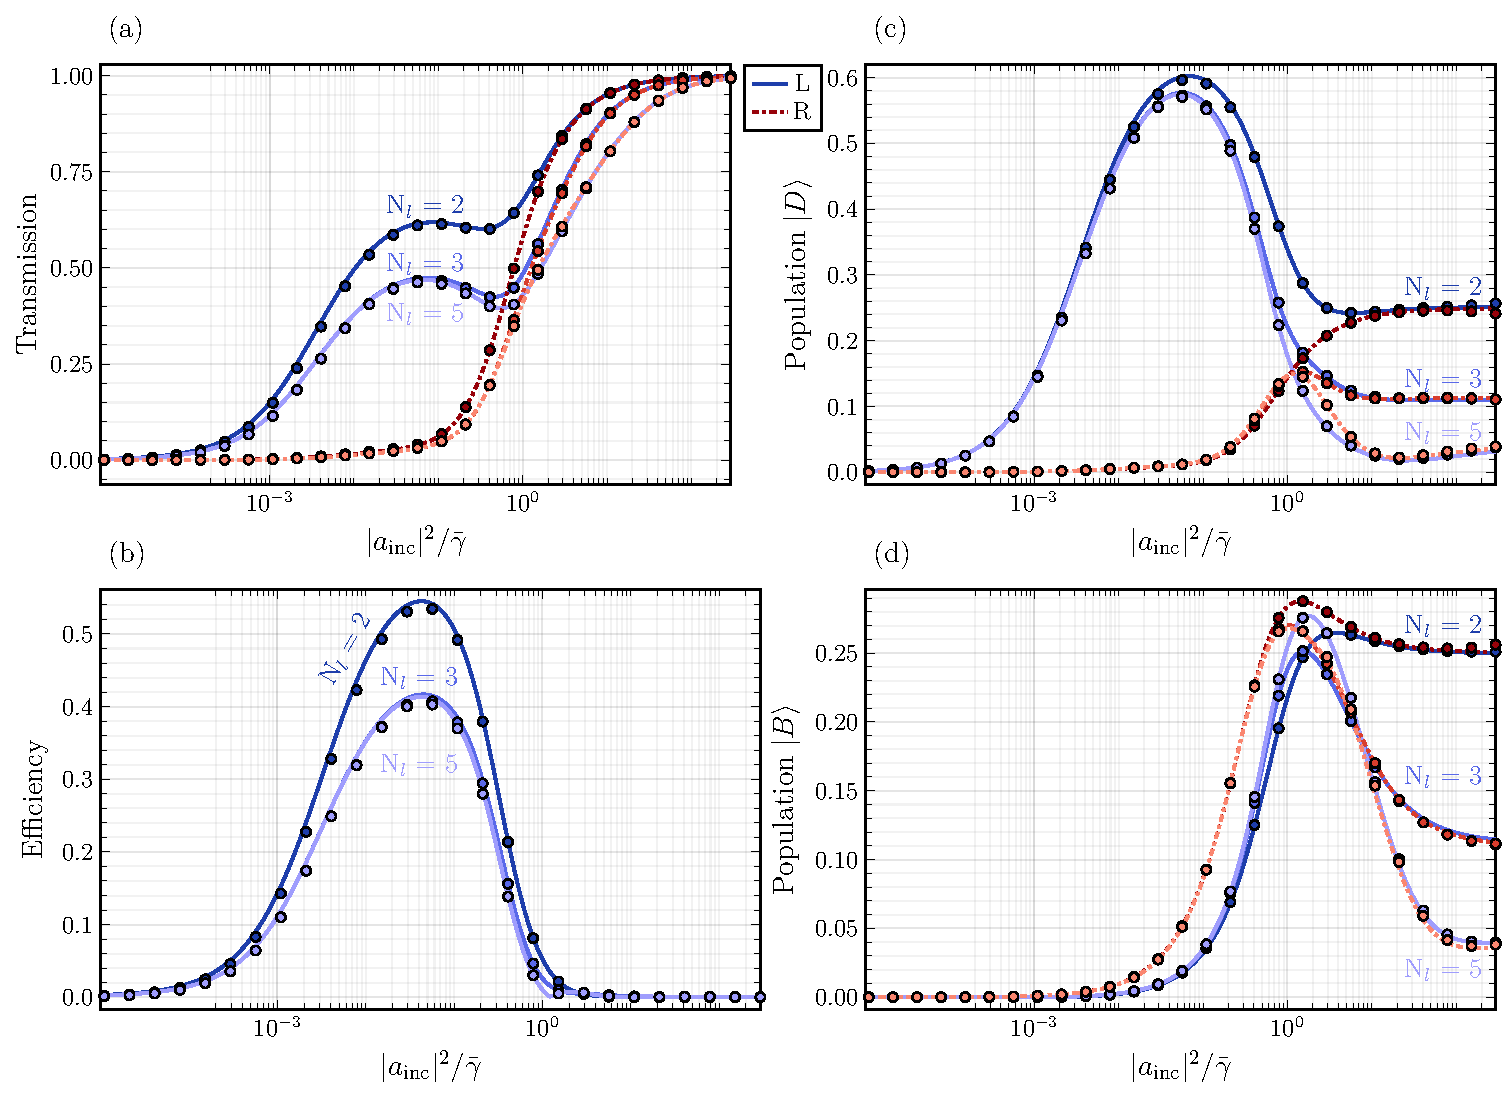
\includegraphics[width=0.85\textwidth]{fig_3_delta-0.15}
    \caption{Incident power ($|a_\mathrm{in}|^2 / \bar{\gamma}$) dependence of (a) transmission for R-propagating waves (red dashed lines) and L-propagating waves (blue solid lines); (b) diode efficiency; the population of the dark state $|D\rangle$ (c) and the bright state $|B\rangle$ (d) in steady-state for R- and L-propagating incident waves. All the plots are made for different numbers of levels in the qubits, namely, $N_l = 2, 3, 5$. The circle markers correspond to the solution without a rotating-wave approximation.}
    \label{fig:03}
\end{figure*}

\subsection{Influence of the higher levels}

Figures~\ref{fig:03}(a,b) also demonstrate how the increase in the number of levels in the qubits affects the nonreciprocity effect, namely, transmission and reflection.
For the R-waves at low powers of excitation, $|a_\mathrm{in}|^2 < \bar{\gamma}$, the transmission behaves despite the number of qubits energy levels.
Namely, the system in this regime reflects the incident waves.
However, the transmission of the L-waves strongly depends on the number of the qubits' energy levels.
For three levels, the transmission and efficiency drop by $\approx 20 \%$ at the low-power excitation regime.
At the same time, populations of the dark and bright states do not change much with the increase in the qubits' energy levels, see Fig.~\ref{fig:03}(c,d).
If we increase the number of levels to five, all the curves, namely, transmissions, efficiencies, and populations, slightly shift towards smaller values.
The changes become negligible for a larger number of levels, and the curves converge fast to the limit ones.

At higher powers of excitation, $|a_\mathrm{in}|^2 > \bar{\gamma}$, the transmission behaviour for both directions of excitation starts depending on the number of levels in the qubits.
All the curves tend to the unity transmission, but with different rates -- the larger the number of levels, the slower transmission approaches unity.
The populations of the dark and bright states also strongly depend on the number of levels in this regime.
The populations decrease with the increase in the levels' number.

Further, we consider a two-parameter space: the power of the incident wave and the Josephson inductance of the first qubit.
Fig.~\ref{fig:05} demonstrates the behaviour of the transmissions and the efficiency in this parametric space.
\begin{figure*}[h]
    \centering
    \includegraphics[width=0.85\textwidth]{fig_5}
    \caption{(a) Diode efficiency for $N_l = 2$ and $N_l = 5$ in the parameter plane of the incident power and Josephson inductance; (b-e) transmissions for R- and L- propagating incident waves at $N_l = 2$ and $N_l = 5$ in the same parameter plane.}
    \label{fig:05}
\end{figure*}
In general, the nonreciprocity effect is sensible to the qubits' detuning.
Therefore, it is also sensible to the difference of the Josephson inductances of the qubits.
In Fig.~\ref{fig:05}, we can see that at low incident powers, we should tune the qubit 1 inductance and, therefore, frequency close to qubit 2 to achieve the nonreciprocity effect.
At larger powers of the incident wave, the restriction for fine-tuning becomes weaker.
Overall, to observe nonreciprocity, one should fulfil the following condition: $\delta < |a_\mathrm{in}|^2 / \bar{\gamma}$, or in other words, the detuning between two qubits should be less than the incident power.

Considering the higher energy levels of qubits does not affect this behaviour.
The power and Josephson inductance dependencies remain the same; see projections in Fig~\ref{fig:05}(a) and Fig.~\ref{fig:05}(b-e); however, the magnitude of the transmission and diode efficiency drops near the resonance for $N_l > 2$.

The reason for such behaviour can be found if we take a close look at the steady-state density matrices of the system.
The diagonal elements of the density matrices in the basis of the dark and bright states for L-wave excitation at $|a_\mathrm{in}|^2 / \bar{\gamma} = 7 \cdot 10^{-2}$ are shown in Fig.~\ref{fig:04}.
\begin{figure}[h!]
    \centering
    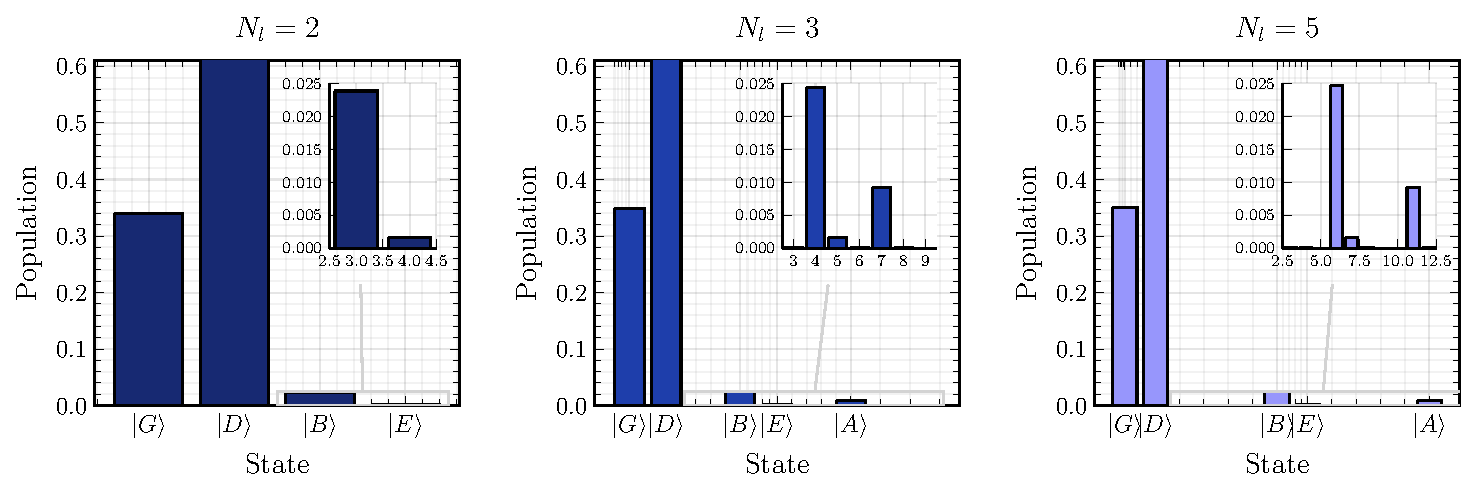
\includegraphics[width=0.48\textwidth]{fig_7}
    \caption{Diagonal elements of the steady-state density matrix in the dark and bright state basis for $N_l = 2, 3, 5$.}
    \label{fig:04}
\end{figure}
In the case of two-level qubits, there are only four states, namely, ground, dark, bright and excited.
As discussed above, only ground and dark states are mainly populated at the nonreciprocity regime for L-wave excitation.
The bright and excited states remain almost unpopulated and do not play a significant role in transmission, as shown in~\cite{muller_nonreciprocal_2017}.
For a two-level qubit, transmission is only determined by the population of the dark state. 
For the present choice of parameters, it is $0.6$, which gives transmission equal $0.6$ as well; see Fig.~\ref{fig:03}(a).
However, if we consider higher levels in the qubits, the steady state does not have a simple form of superposition of the ground and dark states -- higher states are also involved.
In Fig.~\ref{fig:04}, for $N_l = 3$ and $N_l = 5$, an additional state has a nonzero population compared to the two-level case.

We will see two states with nonzero populations if we look closer at the steady-state density matrix at the regime when $\gamma_D < |a_\mathrm{in}|^2 < \gamma_B$.
These states are the symmetric and antisymmetric superposition of $|2,0\rangle$ and $|0, 2\rangle$, and they have the same form as $|D\rangle$ and $|B\rangle$ states.
When $\gamma_1$ and $\gamma_2$ are equal, these states become:
\begin{equation} \label{eq:19}
    \begin{aligned}
        |S/A\rangle =& \frac{1}{\sqrt{2}} \left( |0,2\rangle \pm |2,0\rangle \right).
    \end{aligned}
\end{equation}
Let us consider only the subspace of $|G\rangle$, $|D\rangle$, $|B\rangle$, $|E\rangle$, $|A\rangle$, $|S\rangle$. 
We can plot the transition rates between the states in the chosen subspace; the corresponding transition rate matrix is shown in Fig.~\ref{fig:04_1}(a).
\begin{figure}[h!]
    \centering
    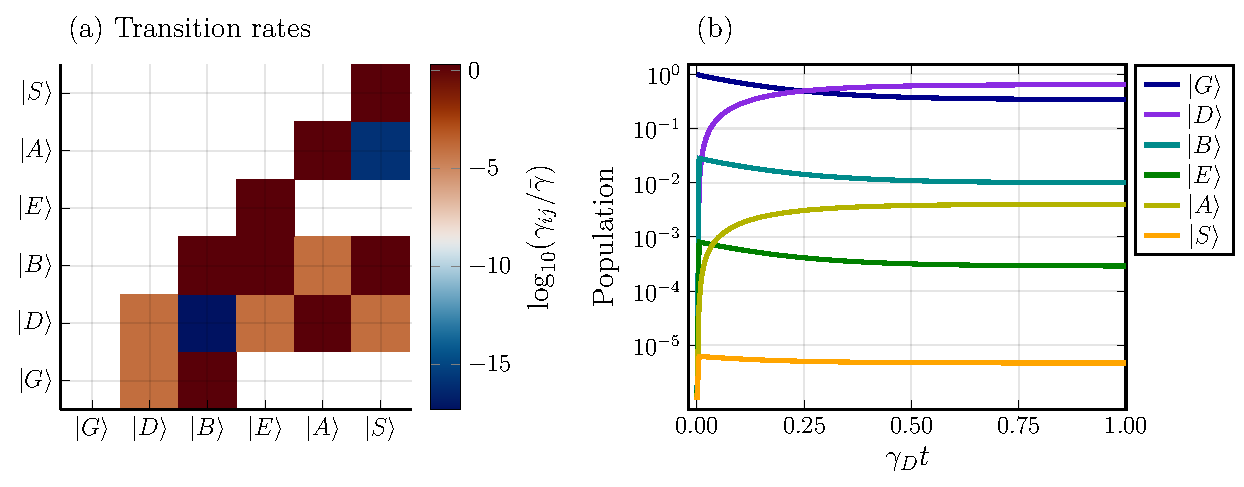
\includegraphics[width=0.48\textwidth]{fig_8}
    \caption{(a) Transition rates between states; (b) states evolution for $N_l = 3$, and $\delta = - 0.015$.}
    \label{fig:04_1}
\end{figure}
\begin{figure*}[h]
    \centering
    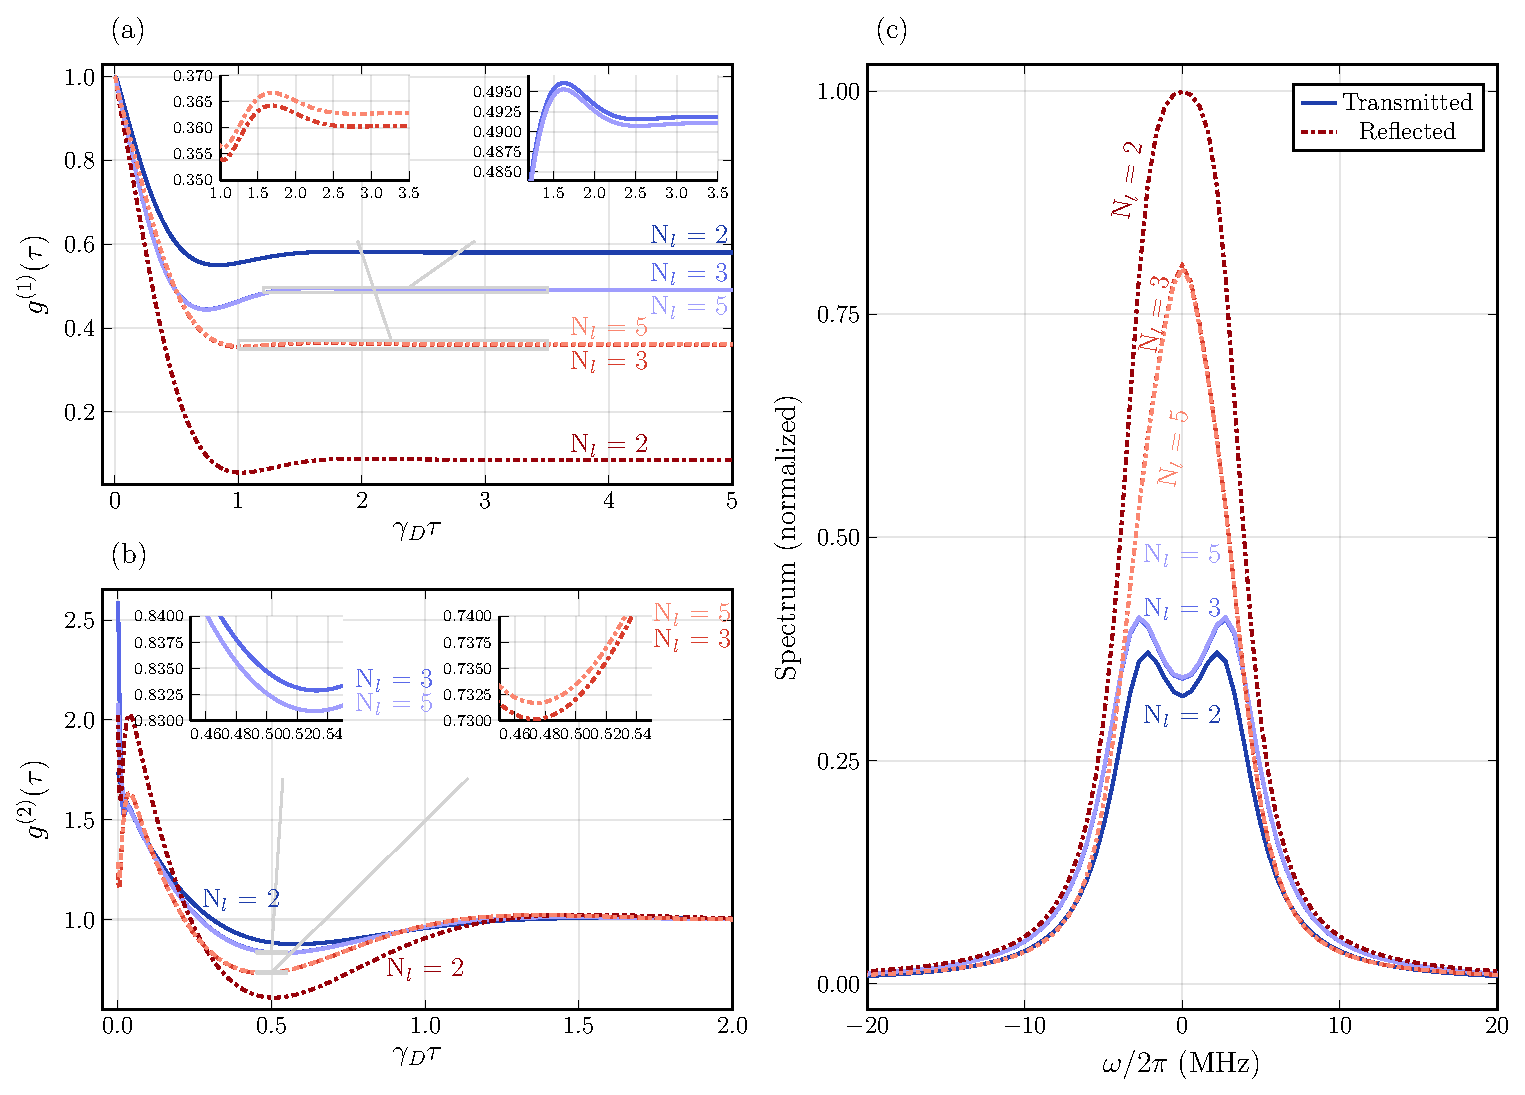
\includegraphics[width=0.85\textwidth]{fig_4_delta-0.15}
    \caption{Comparison for $N_l = 2, 3, 5$ of (a) $g^{(1)}(\tau)$ function, (b) $g^{(2)}(\tau)$ function, (c) power spectrum for transmitted and reflected signals at L-propagating incident wave.}
    \label{fig:06}
\end{figure*}
The transition rate matrix demonstrates additional population transfer channels in the system.
From the symmetric state $|S\rangle$, the population transfers mostly to the bright state $|B\rangle$ and then to the ground state $|G\rangle$.
In contrast, the antisymmetric state feeds mostly the dark state and due to the slow decay rate of the dark state, the population is partially trapped in the $|A\rangle$ state, see Fig.~\ref{fig:04_1}(b).

Thus, the nonzero dipole moments between the symmetric and bright states and between the antisymmetric and dark states lead to the emergence of additional population transfer channels.
These population transfer channels interfere destructively with the main channel, which leads to a reduction in transmission and, consequently, in the diode efficiency.

For more levels included, the structure of the steady-state density matrix is conserved.
Only the values of the dipole moments and populations slightly change.
Therefore, the population transfer channels remain the same as for the three-level case.
Thus, we showed that considering higher levels of qubits leads to the emergence of additional population transfer channels, which interfere destructively with the direct and indirect excitation of the dark state and, consequently, reduce the diode efficiency of the whole system.

\subsection{Spectra and coherence functions depending on number of levels}

In this section, we study the behaviour of the statistical properties of the system, such as $g^{(1)}$ and $g^{(2)}$ functions and the emission spectra and how these properties depend on the number of qubits' energy levels.
These functions are defined as follows:
\begin{equation}\label{eq:20}
    \begin{aligned}
        g^{(1)}_{L,\mathrm{ref}}\left(\tau \right)  &= \frac{\langle (a^{R}_\mathrm{out})^\dag (\tau) a^{R}_\mathrm{out}(0) \rangle}{\langle (a^{R}_\mathrm{out})^+(0) a^{R}_\mathrm{out}(0) \rangle}, \\
        g^{(1)}_{L,\mathrm{trans}}\left(\tau \right)  &= \frac{\langle (a^{L}_\mathrm{out})^\dag (\tau) a^{L}_\mathrm{out}(0) \rangle}{\langle (a^{L}_\mathrm{out})^+(0) a^{L}_\mathrm{out}(0) \rangle}, \\
    \end{aligned}
\end{equation}
\begin{equation}\label{eq:21}
    \begin{aligned}
        g^{(2)}_{L,\mathrm{ref}}\left(\tau \right)  &= \\
        &\frac{\langle (a^{R}_\mathrm{out})^\dag (0) (a^{R}_\mathrm{out})^\dag (\tau) a^{R}_\mathrm{out}(\tau) a^{R}_\mathrm{out}(0)\rangle}{\langle (a^{R}_\mathrm{out})^\dag (t) a^{R}_\mathrm{out}(0) \rangle^2}, \\
        g^{2}_{L,\mathrm{trans}}\left(\tau \right)  &= \\
        &\frac{\langle (a^{L}_\mathrm{out})^\dag (0) (a^{L}_\mathrm{out})^\dag (\tau) a^{L}_\mathrm{out}(\tau) a^{L}_\mathrm{out}(0)\rangle}{\langle (a^{L}_\mathrm{out})^\dag (0) a^{L}_\mathrm{out}(0) \rangle^2}.
    \end{aligned}
\end{equation}

From~\cite{muller_nonreciprocal_2017}, we know that the coherence functions of the first order, $g^{(1)}(\tau)$ have different steady-state depending on the direction of the excitation.
Namely, for the L-wave excitation, the dark state is populated, and, therefore, the coherence function of the transmitted signal in the stationary tends to the value equal to the population of the dark state.
In the ideal case, it is $2/3$.
The coherence function of the reflected signal, in the ideal case, reflects the population of the ground state and tends to $1/3$.

For the R-wave excitation, when the population transfer channels interfere destructively, only the ground state remains populated, and the signal is wholly reflected; therefore, the $g^{(1)}_{R, \mathrm{trans}}(\tau \rightarrow \infty)$ tends to zero.
For the reflected signal the $g^{(1)}_{R, \mathrm{ref}}(\tau \rightarrow \infty)$ remains equal unity.

In Fig.~\ref{fig:06}(a), we see the first-order coherence functions for transmitted and reflected signals at L-wave excitation at powers $\gamma_D < |a_\mathrm{in}|^2 < \gamma_B$, i.e., the dark state becomes populated.
These functions are plotted for the system with realistic parameters (see~\cite{rosario_hamann_nonreciprocity_2018} and Tab.~\ref{tab:01}).
Due to a relatively high detuning between the qubits, $\delta = - 0.15$, the $g^{(1)}_L(\tau)$ functions for transmitted and reflected signals are shifted towards zero, i.e., become less correlated.
However, the transmitted signal's first-order coherence function is still close to the value of the dark state population.

Considering higher energy levels of qubits, we observe that the $g^{(1)}_L(\tau)$ changed significantly.
For the transmitted signal, the coherence function in the stationary reduced its value significantly and moved close to $0.5$.
At the same time, the higher energy levels we consider lower the curve; see the inline plot in Fig.~\ref{fig:06}(a).
On contrary, for the reflected signal, the $g^{(1)}_{L, \mathrm{ref}}(\tau \rightarrow \infty)$ shifted to larger values and became close to $0.4$.
The curves for higher energy levels considered tend to have slightly larger values of the correlation function.

The power spectra
\begin{equation} \label{eq:22}
S(\omega) = \int_{-\infty}^{+\infty} \langle a_\mathrm{out}^\dag(\tau) a_\mathrm{out}(0) \rangle e^{-i \omega \tau} d\tau
\end{equation}
of the output signals from both ports are shown in Fig.~\ref{fig:06}(c).
For the transmitted signal, the spectra demonstrate Rabi splitting because qubit 1 is significantly red-detuned from qubit 2.
The Rabi slitting is less pronounced for the two-level case and becomes more pronounced for $N_l > 2$.
Note that at smaller detunings at the same incident power, Rabi splitting does not occur; also, if we add nonradiative losses and dephasing, Rabi splitting does not emerge.
The reflected signal spectrum does not demonstrate Rabi splitting; however, due to the red detuning, it differs from the Lorentz shape.
The total linewidth for both reflected and transmitted signals is the same and equals $\Gamma_\mathrm{FWHM} \approx 6 \gamma_D$, as shown in ref.~\cite{rosario_hamann_nonreciprocity_2018}.

The $g^{(2)}_L(\tau)$ functions, Eq.~\ref{eq:22}, are shown in Fig.~\ref{fig:06}(b).
At these parameters, Tab.~\ref{tab:01}, the second-order correlation functions for both transmitted and reflected signals vary strongly depending on the number of qubits' energy levels considered.
This behaviour is mainly due to the high detuning between the qubits: the higher states of the system become populated, the dipole moments between these states are induced, and the $g^{(2)}(0)$ function is susceptible to such changes.
However, if we consider an order of magnitude smaller detuning in the system, we will see the real influence of the higher energy levels of qubits.
Fig.~\ref{fig:06_1} shows the second-order coherence functions for a system with smaller detuning, i.e., $\Delta L_J = L_J^{(1)} - L_J^{(2)} = 10^{-3}$ nH and, therefore, the detuning becomes $\delta = -0.015$.
\begin{figure}[h]
    \centering
    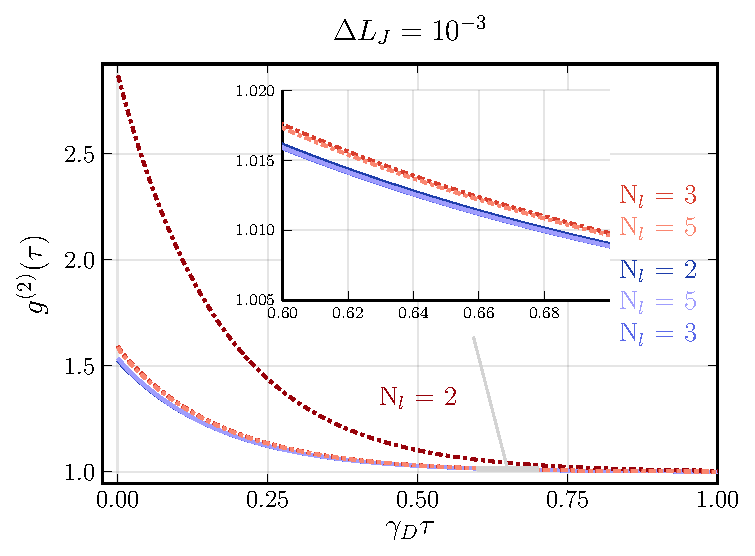
\includegraphics[width=0.45\textwidth]{fig_4_1}
    \caption{Second-order coherence functions $g^{(2)}(\tau)$ for transmitted and reflected signals at L-propagating incident wave. $L_J^{(1)} = 3.301$ nH, $L_J^{(1)} = 3.3$ nH, $\delta = -0.015$.}
    \label{fig:06_1}
\end{figure}
For the two-level case, we expect $g^{(2)}_{L, \mathrm{ref}}(0) = 3$ and $g^{(2)}_{L, \mathrm{trans}}(0) = 1.5$ and w can see this behaviour in Fig.~\ref{fig:06_1}.
However, while the $g^{(2)}_{L, \mathrm{trans}}(0)$ function for the transmitted signal has the same value, if we consider the higher energy levels of qubits, the coherence function for the reflected signal at zero delay shifts close to the one for the transmitted signal and takes the value close to $1.5$.
The relaxation rates, as we also discussed for $g^{(1)}(\tau)$ functions, do not depend on $N_l$.
Thus, considering higher energy levels of qubits, the difference between the transmitted and reflected signals in the second-order coherence functions becomes small, almost negligible compared to the two-level case.
Note that the $g^{(2)}_{L, \mathrm{trans}}(\tau)$ for the transmitted signal does not change with increase in $N_l$.

\section{The role of quantum correlations}

Finally, we discuss the influence of correlations between the qubits on the system's dynamics and the nonreciprocity effect.
For this, from the master equation (\ref{eq:05}), we move to the equations for average values of operators.
For simplicity, we focus on the simplest two-level case, where the creation and annihilation operators become: $a_j \rightarrow \sigma_j$ and $a_j^\dag \rightarrow \sigma_j^+$.
Using the master equation (\ref{eq:05}), we obtain the following system of equations for the average values:
\begin{equation} \label{eq:23}
    \frac{d}{dt}\langle O \rangle = \mathrm{Tr}\left( \dot{\rho} O \right).
\end{equation}
The full description of the system with two-level qubits includes equations for one-operator expectation values and the expectation values for products of two operators, namely, $\langle \sigma_j \rangle$, $\langle \sigma_j^+ \sigma_k \rangle$, $\langle \sigma_j \sigma_k \rangle$, $\langle \sigma_j^{ee} \sigma_k^{ee} \rangle$, $\langle \sigma_j^{ee} \sigma_k \rangle$, where $j,k = 1, 2$.
The system of equations for these variables is equivalent to the master equation (\ref{eq:05}).
However, due to the bulkiness of the system, we do not provide it in the main text.

The Hibert space dimension for two qubits is not too large, and one can directly solve the master equation (\ref{eq:05}) and obtain the complete solution.
However, increasing the number of qubits in the system leads to exponential growth in the dimension of the Hilbert space and a practical inability to solve the master equation for $N \gtrsim 15$ qubits.
A common way to address this challenge and to be able to describe systems composed of hundreds of qubits is to employ the so-called semiclassical (or meanfield) approximation. 
The core idea of this approximation is to neglect quantum correlations between qubits.
Within the semiclassical approximation, one assumes that the expectation value of a product of operators is always factorizable, i.e., $\langle O_j O_k \rangle \approx \langle O_j \rangle \langle O_k \rangle$ for any pair of operators $O_j$ and $O_k$, $j,k = 1, \ldots, N$~\cite{scully1999quantum, carmichael1999statistical}. 
This approximation allows us to describe a system of $N$ qubits by solving a $3N$ coupled differential equations instead of $2^{2N}$. 
In particular, the equations describing the evolution of the system in the semiclassical approximation are 
\begin{align} \label{eq:24}
&\frac{d}{dt} \langle {\sigma}_{k}\rangle  = -\frac{1}{2} {\Gamma}_{k,k} \langle {\sigma}_{k}\rangle  - i \left( {\omega}_{k} - \omega_{d} \right) \langle {\sigma}_{k}\rangle + \nonumber \\
&\underset{j{\ne}i,k}{\overset{N}{\sum}} {\Gamma}_{k,j}  \langle {\sigma}_{k}^{{ee}}\rangle   \langle {\sigma}_{j}\rangle  -\frac{1}{2} \underset{j{\ne}i,k}{\overset{N}{\sum}} {\Gamma}_{k,j}  \langle {\sigma}_{j}\rangle  - \\
&i \left( g^*_{k} + \underset{j{\ne}k}{\overset{N}{\sum}} {\Omega}_{k,j}  \langle {\sigma}_{j}\rangle  \right) + 2 i \underset{j{\ne}k}{\overset{N}{\sum}} {\Omega}_{k,j}  \langle {\sigma}_{k}^{{ee}}\rangle   \langle {\sigma}_{j}\rangle  + 2 i g^*_{k} \langle {\sigma}_{k}^{{ee}}\rangle, \nonumber  \\
&\frac{d}{dt} \langle {\sigma}_{k}^{{ee}}\rangle  = - {\Gamma}_{k,k} \langle {\sigma}_{k}^{{ee}}\rangle  +  i {g}_{k} \langle {\sigma}_{k}\rangle   - i g^*_{k} \langle {\sigma}_{k}^+\rangle - \nonumber \\
&\frac{1}{2} \left( \underset{i{\ne}k}{\overset{N}{\sum}} {\Gamma}_{i,k}  \langle {\sigma}_{i}^+\rangle   \langle {\sigma}_{k}\rangle  + \underset{j{\ne}i,k}{\overset{N}{\sum}} {\Gamma}_{k,j}  \langle {\sigma}_{j}\rangle   \langle {\sigma}_{k}^+\rangle  \right) + \\
&i \underset{i{\ne}k}{\overset{N}{\sum}} {\Omega}_{i,k}  \langle {\sigma}_{i}^+\rangle   \langle {\sigma}_{k}\rangle  - i \underset{j{\ne}k}{\overset{N}{\sum}} {\Omega}_{k,j}  \langle {\sigma}_{j}\rangle   \langle {\sigma}_{k}^+\rangle, \nonumber
\end{align}
where $g_k = i \sqrt{\frac{\gamma_j}{2}} \sqrt{\frac{\omega_d}{\omega_j}} \left[ a_\mathrm{in}^L e^{i \omega_d t_j} + a_\mathrm{in}^R e^{-i \omega_d t_j} \right]$ in RWA, and $\sigma_j^{ee} = \sigma_j^+ \sigma_j$.


\begin{figure*}[t]
    \centering
    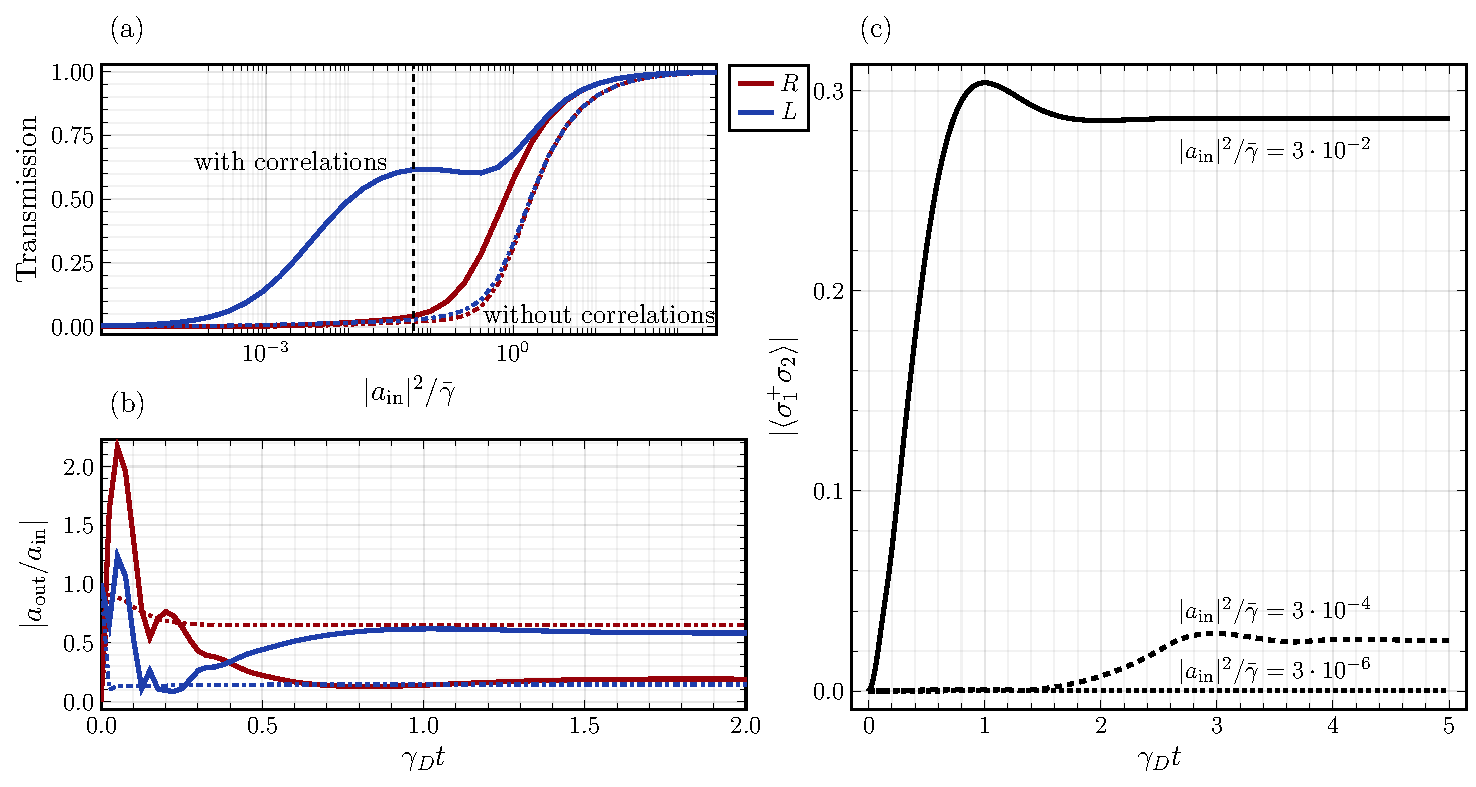
\includegraphics[width=0.85\textwidth]{fig_6}
    \caption{(a) Power dependence of transmissions and (b) time evolution of normalized output signals for R- (red) and L-propagating (blue) incident waves computed with (solid lines) and without (dashed lines) taking into account correlations between qubits for L-wave excitation; (c) correlation between qubits at different incident powers for L-wave excitation.}
    \label{fig:07}
\end{figure*}
In this section, we determine if the semiclassical approximation is valid for describing nonreciprocity in the most straightforward system of two qubits coupled to a 1D waveguide.
We consider the system of two qubits in the transmon regime with parameters listed in Tab.~\ref{tab:01}.
Fig.~\ref{fig:07}(a) demonstrates the power dependence of transmission for R- and L-wave excitation with and without the semiclassical approximation.
We can see that the nonreciprocity in the semiclassical model is not pronounced, and the transmission curves do not approximate the results of the full model.
Note that because the semiclassical equations fulfil the nonreciprocity requirements, namely, broken symmetry and nonlinearity, one can achieve a strong nonreciprocal response from the system utilizing classical nonlinearities~\cite{cotrufo2021nonlinearity1, cotrufo2021nonlinearity2, sounas_fundamental_2018, yang_inverse-designed_2020}, but with entirely different parameter set.

Looking at the evolution of the output signal amplitudes from both channels, Fig.~\ref{fig:07}(b), we see that the output signals behave drastically differently in the full and semiclassical models.
In the semiclassical model, the normalized output signal for the R-wave (reflected signal in the considered case) grows fast from zero to one. 
Then, it tends to the stationary value $\approx 2/3$.
At the same time, the transmitted signal quickly drops from unity and stays at the value $\approx 0.15$.
On the other hand, for the full model, both the reflected and transmitted signals grow at a small time scale.
At the time scale of $\gamma_D^{-1}$, the output signals tend to the stationary values: $0.6$ for the transmitted signal and $0.2$ for the reflected signal.
This slow dynamics at the time scale of the $|D\rangle$-state lifetime happens due to the quantum correlations leading to the constructive interference of the population transfer channels.

The dominating correlations between two qubits in the system are represented by the expectation values of the product of two operators, $\langle \sigma_1^+ \sigma_2 \rangle$.
It has the time scale of $\gamma_D^{-1}$ and gives the main contribution to the transmitted signal:
\begin{equation} \label{eq:25}
\begin{aligned}
    T_L =& 1 + \frac{1}{|a_\mathrm{in}|}\sum_j \sqrt{\gamma_j} \mathrm{Re}\left(\langle \sigma_j \rangle e^{i \omega_j t_j}\right) + \\
    &\frac{1}{|a_\mathrm{in}|^2} \sum_{j,k} \frac{\sqrt{\gamma_j \gamma_k}}{2} \langle \sigma_j^+ \sigma_k \rangle e^{-i (\omega_j t_j - \omega_k t_k)}.
\end{aligned}
\end{equation}
In Fig.~\ref{fig:07}(c), the evolution of $|\langle \sigma_1^+ \sigma_2\rangle |$ is shown.
We can see that at the powers when the nonreciprocity effect is the strongest, the correlation between the qubits is also maximal.
Whereas at smaller incident powers, it becomes negligible.
For instance, at $|a_\mathrm{in}|^2 / \bar{\gamma} = 3\cdot 10^{-6}$, it is almost zero, and the solution of the full model coincides with the one of the semiclassical model.
Thus, the semiclassical model is applicable for the system of two qubits coupled to a waveguide only when the quantum correlations between the qubits are negligible, i.e., at the low incident powers, namely, $|a_\mathrm{in}|^2 < \gamma_D$.
To observe nonreciprocity in such a system, one has to consider the quantum correlations between the qubits because, as we showed above, they play a crucial role in the nature of the whole effect.

\section{Conclusion}

In this work, we have thoroughly examined the behaviour of a system composed of two superconducting qubits in a transmon regime coupled to a 1D waveguide, with a specific focus on the phenomenon of nonreciprocity. 
Nonreciprocity in such and similar systems has been previously documented~\cite{dai_rectification_2015, muller_nonreciprocal_2017, rosario_hamann_nonreciprocity_2018, Nefedkin2022, trivedi_fano-qubits_2023}, and our objective was to investigate the influence of approximations in theoretical models on the observed nonreciprocal effects, as well as to identify critical factors that should be taken into account.
We use the real parameters of the qubits from ref.~\cite{rosario_hamann_nonreciprocity_2018} listed in Tab.~\ref{tab:01}.

Our investigation has revealed that, for qubits operating in a transmon regime characterized by weak anharmonicity, the inclusion of higher energy levels of the qubits leads to noticeable alterations in the system's dynamics. 
Particularly, the nonreciprocity effect diminishes, resulting in reduced values of the diode efficiency. 
Consequently, the efficiency limit falls below $2/3$. 
Furthermore, the statistical properties of the system undergo significant changes. 
The first-order coherent functions for transmitted and reflected signals approach a value of approximately $0.5$ in the stationary state. 
In contrast, in the case of a two-level approximation, these functions assume the values $2/3$ and $1/3$, respectively. 
Additionally, the second-order coherent functions for transmitted and reflected signals become less distinguishable and tend to coincide, as illustrated in Figure~\ref{fig:04_1}.

This behaviour can be attributed to the emergence of two additional population transfer channels associated with the states $|S/A\rangle = 1/\sqrt{2} \left( |0,2\rangle \pm |2,0\rangle \right)$, occurring at moderate incident powers ($\gamma_D < |a_\mathrm{in}|^2 < \gamma_B$). 
These channels interfere destructively with the existing channels, which involve states $|G\rangle$, $|B\rangle$, and $|D\rangle$, resulting in a reduction of the nonreciprocity effect. 
Importantly, this behaviour persists when considering more than three energy levels of the qubits, with only minor quantitative changes in populations, transmissions, and reflections.

Furthermore, our investigation underscores the critical importance of considering quantum correlations between the qubits for an accurate representation of the nonreciprocity effect within the model. 
The semiclassical model, which relies on factorized expectation values of operator products, fails to approximate the system's dynamics adequately. 
This inadequacy arises from the strong correlations, denoted as $\langle \sigma_j^+ \sigma_k \rangle$ for $j\neq k$, induced in the system in the nonreciprocal regime. 
Notably, these correlations weaken at lower incident powers ($|a_\mathrm{in}|^2 < \gamma_D$), enabling the use of the semiclassical approximation within this regime.

These findings provide insights into the intricacies of nonreciprocal quantum systems, with direct implications for practical quantum device engineering. 
For instance, for quantum diodes, understanding the impact of higher energy levels on nonreciprocity can lead to the design of more efficient and versatile devices for signal routing and processing. 
Moreover, our exploration of the role of quantum correlations between qubits underscores the necessity of precision in modelling, which can be leveraged to develop advanced quantum communication systems. 
These insights are pivotal for achieving the full potential of such systems. They will drive the refinement of theoretical models, ultimately enabling the design of more accurate and efficient quantum devices. 


\subsection*{Acknowledgements}
\noindent This should be a simple paragraph before the bibliography to thank those individuals and institutions who have supported your work on this article.



\bibliography{ref}

\begin{IEEEbiographynophoto}{Jane Doe}
Biography text here without a photo.
\end{IEEEbiographynophoto}

% \begin{IEEEbiography}
% In this paragraph, you can place your educational, professional background, research and other interests.
% \end{IEEEbiography}


\end{document}

% \begin{strip}
% \begin{align} \label{eq:23}
% \frac{d}{dt} \langle {\sigma}_{1}\rangle  =& -i \left( g^*_{1} + \Omega_{{1,2}} \langle {\sigma}_{2}\rangle  \right) + \Gamma_{{1,2}} \langle {\sigma}_{1}^{{ee}}  {\sigma}_{2}\rangle  + 2 i g^*_{1} \langle {\sigma}_{1}^{{ee}}\rangle  - \frac{\Gamma_{{1,1}}}{2} \langle {\sigma}_{1}\rangle  - \frac{\Gamma_{{1,2}}}{2} \langle {\sigma}_{2}\rangle  - i \Omega_{{1,1}} \langle {\sigma}_{1}\rangle  + 2 i \Omega_{{1,2}} \langle {\sigma}_{1}^{{ee}}  {\sigma}_{2}\rangle  - i \left( \omega_{1} - \omega_d \right) \langle {\sigma}_{1}\rangle  \\
% \frac{d}{dt} \langle {\sigma}_{2}\rangle  =& - i \left( g^*_{2} + \Omega_{{2,1}} \langle {\sigma}_{1}\rangle  \right) + \Gamma_{{2,1}} \langle {\sigma}_{1}  {\sigma}_{2}^{{ee}}\rangle  -\frac{1}{2} \Gamma_{{2,2}} \langle {\sigma}_{2}\rangle  - i \Omega_{{2,2}} \langle {\sigma}_{2}\rangle  -\frac{1}{2} \Gamma_{{2,1}} \langle {\sigma}_{1}\rangle  + 2 i g^*_{2} \langle {\sigma}_{2}^{{ee}}\rangle  + 2 i \Omega_{{2,1}} \langle {\sigma}_{1}  {\sigma}_{2}^{{ee}}\rangle  - i \left( \omega_{2} -1 \omega_{e x t} \right) \langle {\sigma}_{2}\rangle  \\
% \frac{d}{dt} \langle {\sigma}_{1}  {\sigma}_{2}^+\rangle  =& -\frac{1}{2} \Gamma_{{1,2}} \langle {\sigma}_{2}^{{ee}}\rangle  -\frac{1}{2} \Gamma_{{1,2}} \langle {\sigma}_{1}^{{ee}}\rangle  -\frac{1}{2} \left( \Gamma_{{1,1}} + \Gamma_{{2,2}} \right) \langle {\sigma}_{1}  {\sigma}_{2}^+\rangle  - i \Omega_{{1,2}} \langle {\sigma}_{2}^{{ee}}\rangle  + i g_{2} \langle {\sigma}_{1}\rangle  - i g^*_{1} {\langle {\sigma}_{2}\rangle ^{*}} + 2.0 \Gamma_{{1,2}} \langle {\sigma}_{1}^{{ee}}  {\sigma}_{2}^{{ee}}\rangle  + i \Omega_{{1,2}} \langle {\sigma}_{1}^{{ee}}\rangle  - i \left( \Omega_{{1,1}} + \omega_{1} -1 \omega_{e x t} \right) \langle {\sigma}_{1}  {\sigma}_{2}^+\rangle  + i \left( \Omega_{{2,2}} + \omega_{2} -1 \omega_{e x t} \right) \langle {\sigma}_{1}  {\sigma}_{2}^+\rangle  -2 i g_{2} \langle {\sigma}_{1}  {\sigma}_{2}^{{ee}}\rangle  + 2 i g^*_{1} {\langle {\sigma}_{1}^{{ee}}  {\sigma}_{2}\rangle ^{*}} \\
% \frac{d}{dt} \langle {\sigma}_{1}^{{ee}}\rangle  =& -\frac{1}{2} \left( \Gamma_{{1,2}} {\langle {\sigma}_{1}  {\sigma}_{2}^+\rangle ^{*}} + \Gamma_{{2,1}} \langle {\sigma}_{1}  {\sigma}_{2}^+\rangle  \right) -1.0 \Gamma_{{1,1}} \langle {\sigma}_{1}^{{ee}}\rangle  + i g_{1} \langle {\sigma}_{1}\rangle  + i \Omega_{{2,1}} \langle {\sigma}_{1}  {\sigma}_{2}^+\rangle  - i g^*_{1} {\langle {\sigma}_{1}\rangle ^{*}} - i \Omega_{{1,2}} {\langle {\sigma}_{1}  {\sigma}_{2}^+\rangle ^{*}} \\
% \frac{d}{dt} \langle {\sigma}_{2}^{{ee}}\rangle  =& -\frac{1}{2} \left( \Gamma_{{1,2}} {\langle {\sigma}_{1}  {\sigma}_{2}^+\rangle ^{*}} + \Gamma_{{2,1}} \langle {\sigma}_{1}  {\sigma}_{2}^+\rangle  \right) -1.0 \Gamma_{{2,2}} \langle {\sigma}_{2}^{{ee}}\rangle  + i g_{2} \langle {\sigma}_{2}\rangle  - i \Omega_{{2,1}} \langle {\sigma}_{1}  {\sigma}_{2}^+\rangle  - i g^*_{2} {\langle {\sigma}_{2}\rangle ^{*}} + i \Omega_{{1,2}} {\langle {\sigma}_{1}  {\sigma}_{2}^+\rangle ^{*}} \\
% \frac{d}{dt} \langle {\sigma}_{1}^{{ee}}  {\sigma}_{2}^{{ee}}\rangle  =& \left( -1.0 \Gamma_{{1,1}} -1.0 \Gamma_{{2,2}} \right) \langle {\sigma}_{1}^{{ee}}  {\sigma}_{2}^{{ee}}\rangle  + i g_{1} \langle {\sigma}_{1}  {\sigma}_{2}^{{ee}}\rangle  + i g_{2} \langle {\sigma}_{1}^{{ee}}  {\sigma}_{2}\rangle  - i g^*_{1} {\langle {\sigma}_{1}  {\sigma}_{2}^{{ee}}\rangle ^{*}} - i g^*_{2} {\langle {\sigma}_{1}^{{ee}}  {\sigma}_{2}\rangle ^{*}} \\
% \frac{d}{dt} \langle {\sigma}_{1}  {\sigma}_{2}^{{ee}}\rangle  =& -\frac{1}{2} \Gamma_{{1,2}} \langle {\sigma}_{1}^{{ee}}  {\sigma}_{2}\rangle  + i g_{2} \langle {\sigma}_{1}  {\sigma}_{2}\rangle  - i g^*_{1} \langle {\sigma}_{2}^{{ee}}\rangle  - i g^*_{2} \langle {\sigma}_{1}  {\sigma}_{2}^+\rangle  + i \Omega_{{1,2}} \langle {\sigma}_{1}^{{ee}}  {\sigma}_{2}\rangle  + 2 i g^*_{1} \langle {\sigma}_{1}^{{ee}}  {\sigma}_{2}^{{ee}}\rangle  -\frac{1}{2} \Gamma_{{1,1}} \langle {\sigma}_{1}  {\sigma}_{2}^{{ee}}\rangle  -1.0 \Gamma_{{2,2}} \langle {\sigma}_{1}  {\sigma}_{2}^{{ee}}\rangle  - i \left( \Omega_{{1,1}} + \omega_{1} -1 \omega_{e x t} \right) \langle {\sigma}_{1}  {\sigma}_{2}^{{ee}}\rangle  \\
% \frac{d}{dt} \langle {\sigma}_{1}^{{ee}}  {\sigma}_{2}\rangle  =& - i g^*_{2} \langle {\sigma}_{1}^{{ee}}\rangle  -\frac{1}{2} \Gamma_{{2,2}} \langle {\sigma}_{1}^{{ee}}  {\sigma}_{2}\rangle  + i g_{1} \langle {\sigma}_{1}  {\sigma}_{2}\rangle  -1.0 \Gamma_{{1,1}} \langle {\sigma}_{1}^{{ee}}  {\sigma}_{2}\rangle  + 2 i g^*_{2} \langle {\sigma}_{1}^{{ee}}  {\sigma}_{2}^{{ee}}\rangle  - i \left( \Omega_{{2,2}} + \omega_{2} -1 \omega_{e x t} \right) \langle {\sigma}_{1}^{{ee}}  {\sigma}_{2}\rangle  - i g^*_{1} {\langle {\sigma}_{1}  {\sigma}_{2}^+\rangle ^{*}} -\frac{1}{2} \Gamma_{{2,1}} \langle {\sigma}_{1}  {\sigma}_{2}^{{ee}}\rangle  + i \Omega_{{2,1}} \langle {\sigma}_{1}  {\sigma}_{2}^{{ee}}\rangle  \\
% \frac{d}{dt} \langle {\sigma}_{1}  {\sigma}_{2}\rangle  =& - i g^*_{1} \langle {\sigma}_{2}\rangle  + 2 i g^*_{1} \langle {\sigma}_{1}^{{ee}}  {\sigma}_{2}\rangle  -\frac{1}{2} \left( \Gamma_{{1,1}} + \Gamma_{{2,2}} \right) \langle {\sigma}_{1}  {\sigma}_{2}\rangle  - i g^*_{2} \langle {\sigma}_{1}\rangle  + 2 i g^*_{2} \langle {\sigma}_{1}  {\sigma}_{2}^{{ee}}\rangle  - i \left( \Omega_{{1,1}} + \Omega_{{2,2}} + \omega_{1} + \omega_{2} -2 \omega_{e x t} \right) \langle {\sigma}_{1}  {\sigma}_{2}\rangle 
% \end{align}
% \end{strip}


